% !TEX encoding = UTF-8 Unicode
% !TEX TS-program = xelatex

\chapter{空間向量}

\begin{tikzpicture}[scale=0.6]
\pgfmathsetmacro{\EAlphaVectorX}{8}
\pgfmathsetmacro{\EAlphaVectorY}{0}
\pgfmathsetmacro{\EBetaVectorX}{2}
\pgfmathsetmacro{\EBetaVectorY}{3}

\coordinate (cPPt) at (2.5,1.5);
\coordinate (cQPt) at (7,1.5);
\coordinate (cVectorPP) at (4,4);
\coordinate (cNVector) at (0,5); 
\coordinate (cPPrimePt) at ($(cPPt)+(cVectorPP)$);
\coordinate (cQPrimePt) at ($(cQPt)+(cVectorPP)$);
\coordinate (cNVectorEndPt) at ($(cPPt) + (cNVector)$);

\draw (cPPt)--(cQPt)  node [midway, below ] {$7$};
\draw (cPPrimePt)--(cQPrimePt);
\draw[fill=lightgray] (cPPt)--(cQPt)--(cQPrimePt)--(cPPrimePt)--cycle;
\draw (0,0) -- ++(\EAlphaVectorX, \EAlphaVectorY) -- ++(\EBetaVectorX, \EBetaVectorY) -- ++(-\EAlphaVectorX, -\EAlphaVectorY) -- ++(-\EBetaVectorX, -\EBetaVectorY) -- cycle;
\draw[-{Stealth[scale=1.3,angle'=45]},semithick] (cPPt) -- ++(cVectorPP);
\draw[-{Stealth[scale=1.3,angle'=45]},semithick] (cQPt) -- ++(cVectorPP) ;
\draw[-{Stealth[scale=1.3,angle'=45]},semithick] (cPPt) -- (cNVectorEndPt) ;

\foreach \v/\u/\t in 
{cPPt/270/$P$,
    cQPt/270/$Q$,
    cPPrimePt/90/$P^\prime$,
    cQPrimePt/90/$Q^\prime$,
    cNVectorEndPt/90/$\lvec{n}$
}
{
    %\draw[ultra thick,fill] (\v) circle (2.5pt);
    \node[label=\u:\t] at (\v){};
};
\node[below] at (4,0){$E:3x-2y-2z=1$};
\end{tikzpicture}

\begin{tikzpicture}      
%把空間中的四面體利用平面上的替代點來畫圖
\coordinate (Base1) at (0,0);
\coordinate (Base2) at (5,-1.5);
\coordinate (Base3) at (5,1.5);
\coordinate (TopPt) at (3.5,3.5);
\coordinate (O) at (3.5,0);

\coordinate (S) at (TopPt);
\coordinate (A) at (Base1);
\coordinate (B) at (Base2);
\coordinate (C) at (Base3);
\coordinate (D) at ($(B) !0.5! (C) $);
\coordinate (E) at ($(C) !0.5! (A) $);
\coordinate (F) at ($(A) !0.5! (B) $);


\draw [draw=black, every edge/.append style={draw=black, dashed}]
(Base1) -- (Base2) --(Base3) 
(Base3) edge (Base1);

\draw [draw=black, every edge/.append style={draw=black, dashed}]
(TopPt) -- (Base1) 
(TopPt) -- (Base2) 
(TopPt) -- (Base3)
(TopPt) -- (O)
(S) -- (D)
(S) edge (E)
(S) -- (F)
(O) edge node[sloped] {$\parallel$} (D)
(O) edge node[sloped] {$\parallel$} (E)
(O) edge node[sloped] {$\parallel$} (F);

\foreach \v/\u/\t in 
{ S/90/$S$,
    A/0/$A$,
    B/0/$B$,
    C/0/$C$,
    O/90 /$O$,
    D/0/$D$,
    E/135/$E$,
    F/225/$F$
}
{
    \draw[ultra thick,fill] (\v) circle (1.5pt);
    \node[label=\u:\t] at (\v){};
}; 
\end{tikzpicture}

\begin{tikzpicture}      
%把空間中的四面體利用平面上的替代點來畫圖
\coordinate (Base1) at (0,0);
\coordinate (Base2) at (5,-1.5);
\coordinate (Base3) at (5,1.5);
\coordinate (TopPt) at (3.5,3.5);
\coordinate (O) at (3.5,0);

\coordinate (S) at (TopPt);
\coordinate (A) at (Base1);
\coordinate (B) at (Base2);
\coordinate (C) at (Base3);
\coordinate (D) at ($(B) !0.5! (C) $);
\coordinate (E) at ($(C) !0.5! (A) $);
\coordinate (F) at ($(A) !0.5! (B) $);


\draw [draw=black, every edge/.append style={draw=black, dashed}]
(Base1) -- (Base2) --(Base3) 
(Base3) edge (Base1);

\draw [draw=black, every edge/.append style={draw=black, dashed}]
(TopPt) -- (Base1) 
(TopPt) -- (Base2) 
(TopPt) -- (Base3)
(TopPt) -- (O)
(S) -- (D)
(S) edge (E)
(S) -- (F)
(O) edge node[sloped] {$\parallel$} (D)
(O) edge node[sloped] {$\parallel$} (E)
(O) edge node[sloped] {$\parallel$} (F);

\foreach \v/\u/\t in 
{ S/90/$S$,
    A/0/$A$,
    B/0/$B$,
    C/0/$C$,
    O/90 /$O$,
    D/0/$D$,
    E/135/$E$,
    F/225/$F$
}
{
    \draw[ultra thick,fill] (\v) circle (1.5pt);
    \node[label = \u:\t] at (\v){};
}; 
\end{tikzpicture}



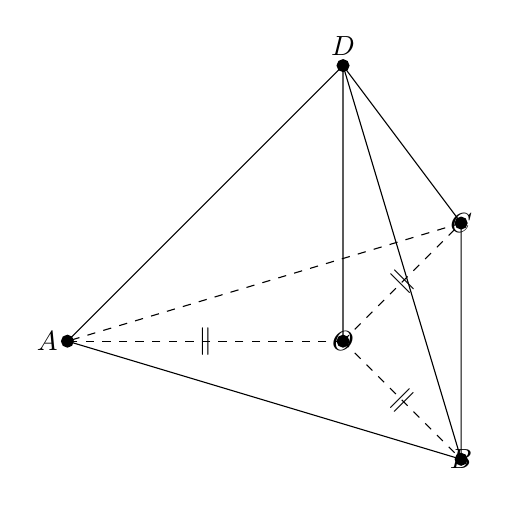
\begin{tikzpicture}      
%把空間中的四面體利用平面上的替代點來畫圖
\coordinate (Base1) at (0,0);
\coordinate (Base2) at (5,-1.5);
\coordinate (Base3) at (5,1.5);
\coordinate (TopPt) at (3.5,3.5);
\coordinate (O) at (3.5,0);

\coordinate (D) at (TopPt);
\coordinate (A) at (Base1);
\coordinate (B) at (Base2);
\coordinate (C) at (Base3);

\draw [draw=black, every edge/.append style={draw=black, dashed}]
(Base1) -- (Base2) --(Base3) 
(Base3) edge (Base1);

\draw [draw=black, every edge/.append style={draw=black, dashed}]
(TopPt) -- (Base1) 
(TopPt) -- (Base2) 
(TopPt) -- (Base3)
(TopPt) -- (O)
(O) edge node[sloped] {$\parallel$} (Base1)
(O) edge node[sloped] {$\parallel$} (Base2)
(O) edge node[sloped] {$\parallel$} (Base3);

\foreach \v/\u/\t in 
{ D/above/$D$,
    A/left/$A$,
    B//$B$,
    C//$C$,
    O//$O$
}
{
    \draw[ultra thick,fill] (\v) circle (1.5pt);
    \node[\u] at (\v){\t};
}; 
\end{tikzpicture}

\vspace{3cm}

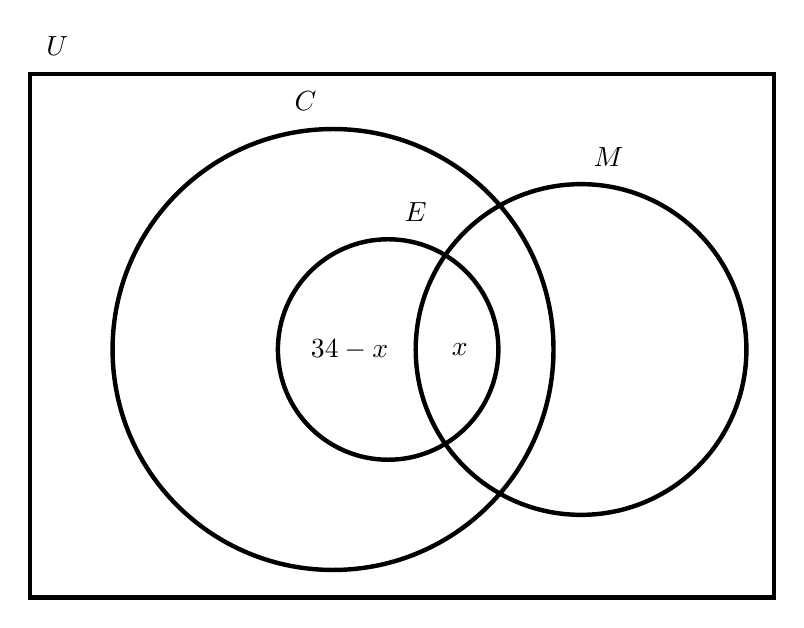
\begin{tikzpicture}[scale=0.7]


\draw[ultra thick]  (-6.5,6) circle (2);
\draw[ultra thick]  (-7.5,6) node (v1) {} ellipse (4 and 4);


\draw[ultra thick]  (-3,6) node (v2) {} circle (3);

\draw[ultra thick]  (-13,11) rectangle (0.5,1.5);

\node at (-12.5,11.5) {$U$};
\node at (-8,10.5) {$C$};

\node at (-5.2,6) {$x$};

\node at (-7.2,6) {$34-x$};
\node at (-6,8.5) {$E$};

\node at (-2.5,9.5) {$M$};

\end{tikzpicture}

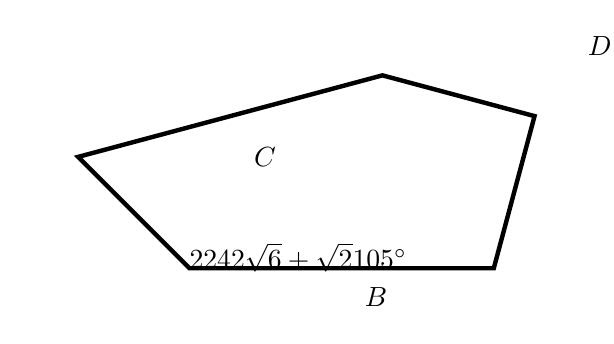
\begin{tikzpicture}[scale=1.0]

\coordinate (B) at (0,0);
\coordinate (A) at (0:{sqrt(6)+sqrt(2)});
\path (A) ++(75:2) coordinate (E);
\path (E) ++(165:2) coordinate (D);
\coordinate (C) at (135:2);


\draw[ultra thick] (A) -- (B)--(C)--(D)--(E) --cycle;
\tkzLabelSegment[midway,  ](E,A){$2$};
\tkzLabelSegment[midway,  above](D,E){$2$};
\tkzLabelSegment[midway,  above](D,C){$4$};
\tkzLabelSegment[midway,  below left](C,B){$2$};
\tkzLabelSegment[midway,  below](B,A){$\sqrt{6}+\sqrt{2}$};
\tkzMarkRightAngle[size=0.3](D,E,A);
\tkzMarkAngle[size=0.3](E,A,B);
\tkzLabelAngle[pos=0.6](E,A,B){$105^\circ$};

\node[label=315:$A$] at (A){};
\node[label=225:$B$] at (B){};
\node[label=180:$C$] at (C){};
\node[label=90:$D$] at (D){};
\node[label=45:$E$] at (E){};
\end{tikzpicture}

\begin{tikzpicture}[every edge quotes/.append style={auto, text=blue},
x={(-0.25cm,-0.15cm)},
y={(0.5cm,0cm)},
z={(0cm,0.5cm)}]

\coordinate (O) at (0,0,0);
\coordinate (x) at (7,0,0);
\coordinate (y) at 
(0,7,0);
\coordinate (z) at (0,0,7);

\coordinate (Base1) at (0,0,0);
\coordinate (Base2) at (6,0,0);
\coordinate (Base3) at (6,6,0);
\coordinate (Base4) at (0,6,0);
\coordinate (Base1Up) at (0,0,6);
\coordinate (Base2Up) at (6,0,6);
\coordinate (Base3Up) at (6,6,6);
\coordinate (Base4Up) at (0,6,6);

\coordinate (A) at (Base2);
\coordinate (B) at (Base3);
\coordinate (C) at (Base4);
\coordinate (D) at (Base4Up);
\coordinate (P) at (0,3,6);
\coordinate (Q) at (3,0,6);
\coordinate (R) at (6,6,3);
\coordinate (S) at (6,0,5);
\coordinate (T) at (0,6,5);


\draw [draw=black, every edge/.append style={draw=black, dashed}]
(Base1) edge (Base2)
(Base2) -- (Base3)
(Base3) -- (Base4)
(Base4) edge (Base1)
(Base1Up) -- (Base2Up)
(Base2Up) -- (Base3Up)
(Base3Up) -- (Base4Up)
(Base4Up) -- (Base1Up)
(Base1) edge (Base1Up)
(Base2) -- (Base2Up)
(Base3) -- (Base3Up)
(Base4) -- (Base4Up);

\draw [fill,pattern=north west lines] (P)--(Q)--(S)--(R)--(T) -- cycle;

\foreach \v/\u/\t in 
{ P/left/$P$,
    Q/below/$Q$,
    R//$R$,
    S/left/$S$,
    T/left/$T$
}
{
    \draw[ultra thick,fill] (\v) circle (1.5pt);
    %\node[\u] at (\v){\t};
}; 

\end{tikzpicture}


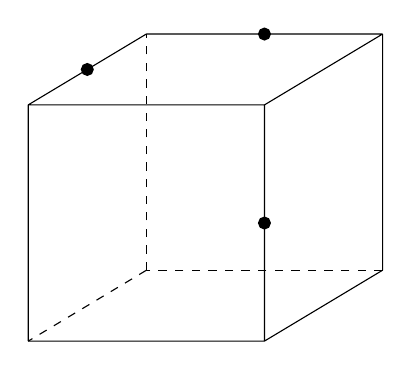
\begin{tikzpicture}[every edge quotes/.append style={auto, text=blue},
x={(-0.25cm,-0.15cm)},
y={(0.5cm,0cm)},
z={(0cm,0.5cm)}]

\coordinate (O) at (0,0,0);
\coordinate (x) at (7,0,0);
\coordinate (y) at 
(0,7,0);
\coordinate (z) at (0,0,7);

\coordinate (Base1) at (0,0,0);
\coordinate (Base2) at (6,0,0);
\coordinate (Base3) at (6,6,0);
\coordinate (Base4) at (0,6,0);
\coordinate (Base1Up) at (0,0,6);
\coordinate (Base2Up) at (6,0,6);
\coordinate (Base3Up) at (6,6,6);
\coordinate (Base4Up) at (0,6,6);

\coordinate (A) at (Base2);
\coordinate (B) at (Base3);
\coordinate (C) at (Base4);
\coordinate (D) at (Base4Up);
\coordinate (P) at (0,3,6);
\coordinate (Q) at (3,0,6);
\coordinate (R) at (6,6,3);
\coordinate (S) at (6,0,5);
\coordinate (T) at (0,6,5);


\draw [draw=black, every edge/.append style={draw=black, dashed}]
(Base1) edge (Base2)
(Base2) -- (Base3)
(Base3) -- (Base4)
(Base4) edge (Base1)
(Base1Up) -- (Base2Up)
(Base2Up) -- (Base3Up)
(Base3Up) -- (Base4Up)
(Base4Up) -- (Base1Up)
(Base1) edge (Base1Up)
(Base2) -- (Base2Up)
(Base3) -- (Base3Up)
(Base4) -- (Base4Up);

%\draw [fill,pattern=north west lines] (P)--(Q)--(S)--(R)--(T) -- cycle;

\foreach \v/\u/\t in 
{ P/left/$P$,
    Q/below/$Q$,
    R//$R$
}
{
    \draw[ultra thick,fill] (\v) circle (1.5pt);
    %\node[\u] at (\v){\t};
}; 

\end{tikzpicture}

   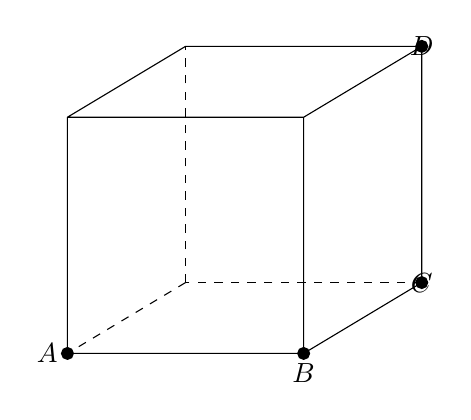
\begin{tikzpicture}[every edge quotes/.append style={auto, text=blue},
   x={(-0.25cm,-0.15cm)},
   y={(0.5cm,0cm)},
   z={(0cm,0.5cm)}]
   %%空間坐標中的CUBE 是以平面上的x軸 y軸再去擴充出深度z軸 z 往前為正,向後為負
   \coordinate (O) at (0,0,0);
   \coordinate (x) at (7,0,0);
   \coordinate (y) at 
   (0,7,0);
   \coordinate (z) at (0,0,7);
   
   \coordinate (Base1) at (0,0,0);
   \coordinate (Base2) at (6,0,0);
   \coordinate (Base3) at (6,6,0);
   \coordinate (Base4) at (0,6,0);
   \coordinate (Base1Up) at (0,0,6);
   \coordinate (Base2Up) at (6,0,6);
   \coordinate (Base3Up) at (6,6,6);
   \coordinate (Base4Up) at (0,6,6);
   
   \coordinate (A) at (Base2);
   \coordinate (B) at (Base3);
   \coordinate (C) at (Base4);
   \coordinate (D) at (Base4Up);
   
   \draw [draw=black, every edge/.append style={draw=black, dashed}]
   (Base1) edge (Base2)
   (Base2) -- (Base3)
   (Base3) -- (Base4)
   (Base4) edge (Base1)
   (Base1Up) -- (Base2Up)
   (Base2Up) -- (Base3Up)
   (Base3Up) -- (Base4Up)
   (Base4Up) -- (Base1Up)
   (Base1) edge (Base1Up)
   (Base2) -- (Base2Up)
   (Base3) -- (Base3Up)
   (Base4) -- (Base4Up);
   
   
   \foreach \v/\u/\t in 
   { A/left/$A$,
       B/below/$B$,
       C//$C$,
       D//$D$
   }
   {
       \draw[ultra thick,fill] (\v) circle (1.5pt);
       \node[\u] at (\v){\t};
   }; 
   
   \end{tikzpicture}
   
  \begin{tikzpicture}[every edge quotes/.append style={auto, text=blue},z={(0cm,0.5cm)},y={(0.5cm,0cm)}, x={(-0.15cm,-0.25cm)}]
   
   %%空間坐標中的CUBE 是以平面上的x軸 y軸再去擴充出深度z軸 z 往前為正,向後為負
   \coordinate (O) at (0,0,0);
   \coordinate (x) at (7,0,0);
   \coordinate (y) at 
   (0,7,0);
   \coordinate (z) at (0,0,7);
   
   \coordinate (Base1) at (0,0,0);
   \coordinate (Base2) at (6,0,0);
   \coordinate (Base3) at (6,6,0);
   \coordinate (Base4) at (0,6,0);
   \coordinate (Base1Up) at (0,0,6);
   \coordinate (Base2Up) at (6,0,6);
   \coordinate (Base3Up) at (6,6,6);
   \coordinate (Base4Up) at (0,6,6);
   
   \coordinate (A) at (Base2);
   \coordinate (B) at (Base4);
   \coordinate (C) at (Base3Up);
   \coordinate (D) at (Base1);
   \coordinate (O) at (3,3,3);
   
   %\coordinate (P) at ($(D)!0.5!(A)$);
   
   \draw [-{Stealth[scale=1.3,angle'=45]},semithick] (D) -- ++(3,0,0) -- ++(0,3,0) -- ++ (0,0,3);
   
   \draw [draw=black, every edge/.append style={draw=black, dashed}]
   (Base1) edge (Base2)
   (Base2) -- (Base3)
   (Base3) -- (Base4)
   (Base4) edge (Base1)
   (Base1Up) -- (Base2Up)
   (Base2Up) -- (Base3Up)
   (Base3Up) -- (Base4Up)
   (Base4Up) -- (Base1Up)
   (Base1) edge (Base1Up)
   (Base2) -- (Base2Up)
   (Base3) -- (Base3Up)
   (Base4) -- (Base4Up);
   
   \foreach \v/\u/\t in 
   { A/180/$A$,
       B/0/$B$,
       C/0/$C$,
       D/180/$D$,
       O/270/$O$
   }
   {
       \draw[ultra thick,fill] (\v) circle (1.5pt);
       \node[label = \u:\t] at (\v){};
   }; 
   
   \end{tikzpicture}
   四面體
   
      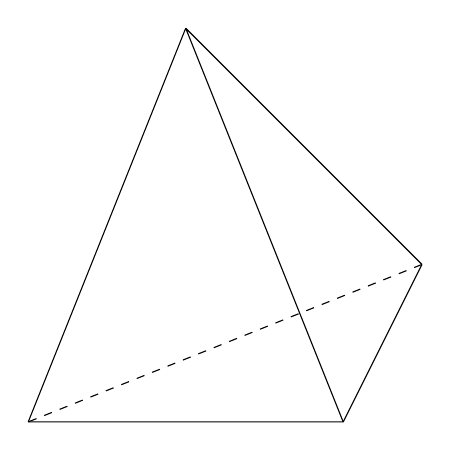
\begin{tikzpicture}      
      %把空間中的四面體利用平面上的替代點來畫圖
      \coordinate (Base1) at (0,0);
      \coordinate (Base2) at (4,0);
      \coordinate (Base3) at (5,2);
      \coordinate (TopPt) at (2,5);
      
      \draw [draw=black, every edge/.append style={draw=black, dashed}]
      (Base1) -- (Base2) --(Base3) 
      (Base3) edge (Base1);
      
      \draw [draw=black, every edge/.append style={draw=black, dashed}]
      (TopPt) -- (Base1) 
      (TopPt) -- (Base2) 
      (TopPt) -- (Base3);
      \end{tikzpicture}
      
            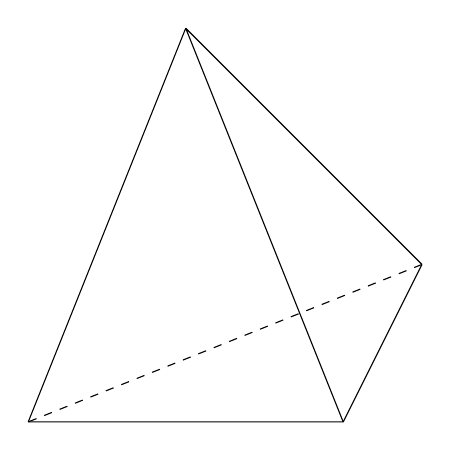
\begin{tikzpicture}      
            %把空間中的四面體利用平面上的替代點來畫圖
            \coordinate (Base1) at (0,0);
            \coordinate (Base2) at (4,0);
            \coordinate (Base3) at (5,2);
            \coordinate (TopPt) at (2,5);
            
            \draw [draw=black, every edge/.append style={draw=black, dashed}]
            (Base1) -- (Base2) --(Base3) 
            (Base3) edge (Base1);
            
            \draw [draw=black, every edge/.append style={draw=black, dashed}]
            (TopPt) -- (Base1) 
            (TopPt) -- (Base2) 
            (TopPt) -- (Base3);
            \end{tikzpicture}
      
        \begin{tikzpicture}      
        %把空間中的四面體利用平面上的替代點來畫圖
        \coordinate (Base1) at (0,0);
        \coordinate (Base2) at (5,-1.5);
        \coordinate (Base3) at (5,1.5);
        \coordinate (TopPt) at (3.5,3.5);
        \coordinate (H) at (3.5,0);
        
        \coordinate (D) at (TopPt);
        \coordinate (A) at (Base1);
        \coordinate (B) at (Base2);
        \coordinate (C) at (Base3);
        \coordinate (M) at ($(A)!0.5!(C)$);
        \coordinate (P) at ($(D)!0.66!(M)$);
        
        \draw [draw=black, every edge/.append style={draw=black, dashed}]
        (Base1) -- (Base2) --(Base3) 
        (Base3) edge (Base1);
        
        \draw [draw=black, every edge/.append style={draw=black, dashed}]
        (TopPt) -- (Base1) 
        (TopPt) -- (Base2) 
        (TopPt) -- (Base3)
        (B) edge (P)
        (P) edge (D);
        
        \foreach \v/\u/\t in 
        { D/above/$D$,
            A/left/$A$,
            B//$B$,
            C//$C$,
            P/left/$P$
        }
        {
            \draw[ultra thick,fill] (\v) circle (1.5pt);
            \node[\u] at (\v){\t};
        }; 
        \end{tikzpicture}

      \begin{tikzpicture}      
      %把空間中的四面體利用平面上的替代點來畫圖
      \coordinate (Base1) at (0,0);
      \coordinate (Base2) at (4,0);
      \coordinate (Base3) at (5,2);
      \coordinate (TopPt) at (2,5);
      
      \coordinate (x) at (6,0);
      
      \coordinate (A) at (TopPt);
      \coordinate (O) at (Base1);
      \coordinate (B) at (Base2);
      \coordinate (C) at (Base3);
      
      \coordinate (M) at ($(B)!0.5!(C)$);
      \coordinate (G) at ($(A)!0.66!(M)$);
      \coordinate (K) at 
      ($(O)!0.66!(B)$);

      \tkzMarkRightAngle(G,K,O)
      \tkzMarkRightAngle(O,G,B)
            
      
      \draw [draw=black, every edge/.append style={draw=black, dashed}]
      (Base1) -- (Base2) --(Base3) 
      (Base3) edge (Base1);
      
      \draw [draw=black, every edge/.append style={draw=black, dashed}]
      (TopPt) -- (Base1) 
      (TopPt) -- (Base2) 
      (TopPt) -- (Base3)
      (A) -- (M)
      (O) edge (G)
      (G) -- (B)
      (G) edge (K);
      
      \draw [-{Stealth[scale=1.3,angle'=45]},semithick] (O) -- (x);
      
      \foreach \v/\u/\t in 
      { A/above/$A$,
          O/left/$O$,
          B/below/$B$,
          C//$C$,
          M//$M$,
          G//$G$,
          K/below/$K$
        }
        {
            \draw[ultra thick,fill] (\v) circle (1.5pt);
            \node[\u] at (\v){\t};
        }; 
        \node[] at (x){$x$};

        \end{tikzpicture}

      \begin{tikzpicture}      
      %把空間中的四面體利用平面上的替代點來畫圖
      \coordinate (Base1) at (0,0);
      \coordinate (Base2) at (4,0);
      \coordinate (Base3) at (5,2);
      \coordinate (TopPt) at (2,5);
      
      \coordinate (A) at (TopPt);
      \coordinate (B) at (Base1);
      \coordinate (C) at (Base2);
      \coordinate (D) at (Base3);
      
      \coordinate (M) at ($(C)!0.5!(D)$);
         
      \draw [draw=black, every edge/.append style={draw=black, dashed}]
      (Base1) -- (Base2) --(Base3) 
      (Base3) edge (Base1);
      
      \draw [draw=black, every edge/.append style={draw=black, dashed}]
      (TopPt) -- (Base1) 
      (TopPt) -- (Base2) 
      (TopPt) -- (Base3);
      
      \draw [ultra thick] (A) -- (M) -- (B)--cycle;
        \foreach \v/\u/\t in 
        { A/above/$A$,
         B/left/$B$,
         C//$C$,
         D//$D$,
         M//$M$
        }
        {
            \draw[ultra thick,fill] (\v) circle (1.5pt);
            \node[\u] at (\v){\t};
        }; 
      \end{tikzpicture}
        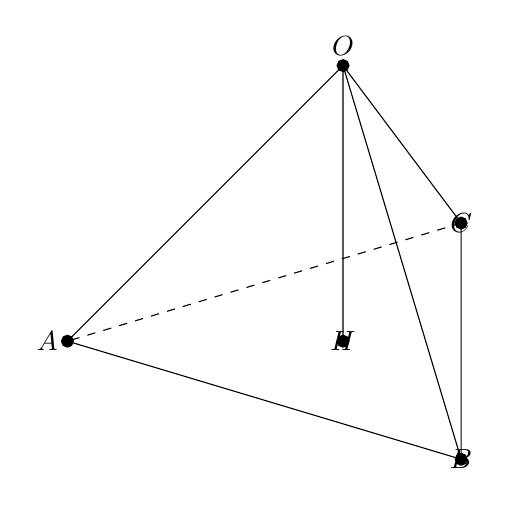
\begin{tikzpicture}      
        %把空間中的四面體利用平面上的替代點來畫圖
        \coordinate (Base1) at (0,0);
        \coordinate (Base2) at (5,-1.5);
        \coordinate (Base3) at (5,1.5);
        \coordinate (TopPt) at (3.5,3.5);
        \coordinate (H) at (3.5,0);
        
        \coordinate (O) at (TopPt);
        \coordinate (A) at (Base1);
        \coordinate (B) at (Base2);
        \coordinate (C) at (Base3);
        
        \draw [draw=black, every edge/.append style={draw=black, dashed}]
        (Base1) -- (Base2) --(Base3) 
        (Base3) edge (Base1);
        
        \draw [draw=black, every edge/.append style={draw=black, dashed}]
        (TopPt) -- (Base1) 
        (TopPt) -- (Base2) 
        (TopPt) -- (Base3)
        (TopPt) -- (H);

        \foreach \v/\u/\t in 
        { O/above/$O$,
            A/left/$A$,
            B//$B$,
            C//$C$,
            H//$H$
        }
        {
            \draw[ultra thick,fill] (\v) circle (1.5pt);
            \node[\u] at (\v){\t};
        }; 
        \end{tikzpicture}
        \begin{tikzpicture}      
        %把空間中的四面體利用平面上的替代點來畫圖
        \coordinate (Base1) at (0,0);
        \coordinate (Base2) at (3,-2);
        \coordinate (Base3) at (5,0);
        \coordinate (TopPt) at (2,3.5);
        \coordinate (H) at (2,-0.55);
        
        \coordinate (O) at (TopPt);
        \coordinate (A) at (Base1);
        \coordinate (B) at (Base2);
        \coordinate (C) at (Base3);
        \coordinate (P) at ($(O)!0.3!(A)$);

        
        \draw [draw=black, every edge/.append style={draw=black, dashed}]
        (Base1) -- (Base2) --(Base3) 
        (Base3) edge (Base1);
        
        \draw [draw=black, every edge/.append style={draw=black, dashed}]
        (TopPt) -- (Base1) 
        (TopPt) -- (Base2) 
        (TopPt) -- (Base3)
        (TopPt) -- (H);
        
        %\draw [ultra thick] (A) -- (M) -- (B)--cycle;
        \foreach \v/\u/\t in 
        { O/above/$O$,
            A/left/$A$,
            B//$B$,
            C//$C$,
            H//$H$,
            P/left/$P$
        }
        {
            \draw[ultra thick,fill] (\v) circle (1.5pt);
            \node[\u] at (\v){\t};
        }; 
        \end{tikzpicture}
        
        Test\\
           \begin{tikzpicture}[every edge quotes/.append style={auto, text=blue},z={(0cm,1cm)},y={(1cm,0cm)}, x={(-0.3cm,-0.3cm)}]

           %%空間坐標中的CUBE 是以平面上的x軸 y軸再去擴充出深度z軸 z 往前為正,向後為負
           \coordinate (A) at (0,0,0);
           \coordinate (B) at (0,4,0);
           \coordinate (C) at (2.5,2.8,0);
           
            \coordinate (A1) at (0,0,3);
            \coordinate (B1) at (0,4,3);
            \coordinate (C1) at (2.5,2.8,3);
            
            \coordinate (D) at ($(A1)!0.5!(B1)$);
            \coordinate (E) at ($(A1)!0.5!(C1)$);

           \draw [draw=black, every edge/.append style={draw=black, dashed}]
           (A) edge (B)
           (A)--(C)
           (B)--(C)
           (A1)--(B1)
           (A1)--(C1)
           (B1)--(C1)
           (A) --(A1)
           (B) --(B1)
           (C) --(C1)
           (A) -- (E)
           (B) edge (D);
           
           
           \foreach \v/\u/\t in 
           { A/left/$A$,
               A1/left/$A_1$,
               B//$B$,
               B1//$B_1$,
               C/below left/$C$,
               C1/below left/$C_1$,
               D/above/$D$,
               E/below/$E$
            }
            {
                \draw[ultra thick,fill] (\v) circle (1.5pt);
                \node[\u] at (\v){\t};
            }; 

            \end{tikzpicture}
           \begin{tikzpicture}[every edge quotes/.append style={auto, text=blue},z={(0cm,1cm)},y={(1cm,0cm)}, x={(-0.3cm,-0.5cm)}]
           

           %%空間坐標中的CUBE 是以平面上的x軸 y軸再去擴充出深度z軸 z 往前為正,向後為負
           \coordinate (O) at (0,0,0);
           \coordinate (x) at (7,0,0);
           \coordinate (y) at 
           (0,6,0);
           \coordinate (z) at (0,0,5);
           \coordinate (B) at (6,0,0);
           \coordinate (C) at (3, {sqrt(27)},0);
           \coordinate (M) at ($(O)!0.5!(B)$);
           \coordinate (G) at ($(M)!0.33!(C)$);
           \coordinate (A) at (3, {sqrt(3)}, {sqrt(24)});
           \draw [draw=black, every edge/.append style={draw=black, dashed}]
           (O) edge (A)
           (O) -- (B)
           (O) edge (C)
           (A) -- (B)
           (A) -- (C)
           (B) -- (C)
           (M) edge (C)
           (G) edge (A); 
           \draw [-{Stealth[scale=1.3,angle'=45]},semithick] (O) -- (x);
           \draw [-{Stealth[scale=1.3,angle'=45]},semithick] (O) -- (y);
           \draw [-{Stealth[scale=1.3,angle'=45]},semithick] (O) -- (z);
           
      \foreach \v/\u/\t in 
      { A/90/$A$,
          O/270/$O$,
          B/180/$B$,
          C/270 /$C$,
          M/270 /$M$,
          G/270 /$G$
        }
        {
            \draw[ultra thick,fill] (\v) circle (1.5pt);
            \node[label = \u:\t] at (\v){};
        }; 
        \node[below left] at (x){$x$};
        \node[] at (y){$y$};
        \node[above] at (z){$z$};
        \tkzMarkRightAngle(O,M,C)
        \tkzMarkRightAngle(A,G,C)
           \end{tikzpicture}
   四角錐\\
   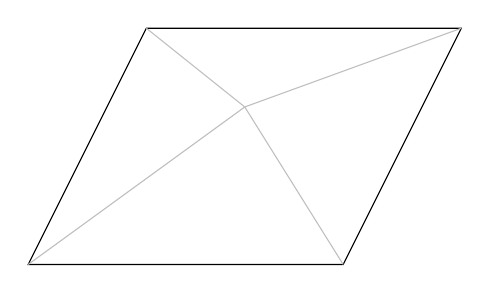
\begin{tikzpicture}[every edge quotes/.append style={auto, text=blue},y={(0cm,1cm)},x={(1cm,0cm)}, z={(-0.25cm,-0.5cm)}]
        
       \pgfmathsetmacro{\sizeEdge}{4}
       \pgfmathsetmacro{\sizeEdgeZ}{6}
       
       \pgfmathsetmacro{\sizeHigh}{0.5}

       %%空間坐標中的CUBE 是以平面上的x軸 y軸再去擴充出深度z軸 z 往前為正,向後為負
       \coordinate (Base1) at (0,0,0);
       \coordinate (Base2) at (0,0, \sizeEdgeZ);
       \coordinate (Base3) at (\sizeEdge,0,\sizeEdgeZ);
       \coordinate (Base4) at (\sizeEdge,0,0);
       \coordinate (TopPt) at (0.5 *\sizeEdge, \sizeHigh, 0.5 * \sizeEdgeZ);
       
       \draw [draw=black, every edge/.append style={draw=black, dashed}]
       (Base1) -- (Base2) --(Base3) --(Base4) -- cycle;
       \draw [draw=lightgray, every edge/.append style={draw=black, dashed}]
       (TopPt) -- (Base1) 
       (TopPt) -- (Base2) 
       (TopPt) -- (Base3)
       (TopPt) -- (Base4);
    \end{tikzpicture}
    
       \begin{tikzpicture}[every edge quotes/.append style={auto, text=blue},y={(0cm,1cm)},x={(1cm,0cm)}, z={(-0.25cm,-0.5cm)}]
       
       \pgfmathsetmacro{\sizeEdge}{4}
       \pgfmathsetmacro{\sizeEdgeZ}{6}
       
       \pgfmathsetmacro{\sizeHigh}{0.5}
       
       %%空間坐標中的CUBE 是以平面上的x軸 y軸再去擴充出深度z軸 z 往前為正,向後為負
       \coordinate (Base1) at (0,0,0);
       \coordinate (Base2) at (0,0, \sizeEdgeZ);
       \coordinate (Base3) at (\sizeEdge,0,\sizeEdgeZ);
       \coordinate (Base4) at (\sizeEdge,0,0);
       \coordinate (TopPt) at (0.5 *\sizeEdge, \sizeHigh, 0.5 * \sizeEdgeZ);
       
       
       \coordinate (D) at (Base1); 
       \coordinate (A) at (Base2);
       \coordinate (B) at (Base3);
       \coordinate (C) at (Base4);
       \coordinate (P) at (TopPt);
       
       \coordinate (O) at ($ (A) !0.5! (C)$);
       \coordinate (M) at ($ (B) !0.5! (C)$);
       
       
       \draw [draw=black, every edge/.append style={draw=black, dashed}]
       (Base1) -- (Base2) --(Base3) --(Base4) -- cycle;
       \draw [draw=lightgray, every edge/.append style={draw=black, dashed}]
       (TopPt) -- (Base1) 
       (TopPt) -- (Base2) 
       (TopPt) -- (Base3)
       (TopPt) -- (Base4);
       \draw [draw=black, every edge/.append style={draw=black, dashed}, ultra thick]
       (P) -- (O) -- (M) -- cycle;
       
       
       \foreach \v/\u/\t in 
       { A/left/$A$,
         B//$B$,
         C//$C$,
         D/left/$D$,
         O/below/$O$,
         P/above/$P$,
         M//$M$
        }
        {
            \draw[ultra thick,fill] (\v) circle (1.5pt);
            \node[\u] at (\v){\t};
        };     
       
       \end{tikzpicture}
       
       \begin{tikzpicture}[every edge quotes/.append style={auto, text=blue},y={(0cm,1cm)},x={(1cm,0cm)}, z={(-0.25cm,-0.5cm)}]
       
       \pgfmathsetmacro{\sizeEdge}{4}
       \pgfmathsetmacro{\sizeEdgeZ}{6}
       
       \pgfmathsetmacro{\sizeHigh}{0.5}
       
       %%空間坐標中的CUBE 是以平面上的x軸 y軸再去擴充出深度z軸 z 往前為正,向後為負
       \coordinate (Base1) at (0,0,0);
       \coordinate (Base2) at (0,0, \sizeEdgeZ);
       \coordinate (Base3) at (\sizeEdge,0,\sizeEdgeZ);
       \coordinate (Base4) at (\sizeEdge,0,0);
       \coordinate (TopPt) at (0.5 *\sizeEdge, \sizeHigh, 0.5 * \sizeEdgeZ);
       
       
       \coordinate (D) at (Base1); 
       \coordinate (A) at (Base2);
       \coordinate (B) at (Base3);
       \coordinate (C) at (Base4);
       \coordinate (P) at (TopPt);
       
       \coordinate (O) at ($ (A) !0.5! (C)$);
       \coordinate (M) at ($ (B) !0.5! (C)$);
       \coordinate (N) at ($ (P) !0.75! (B)$);
       
       
       \draw [draw=black, every edge/.append style={draw=black, dashed}]
       (Base1) -- (Base2) --(Base3) --(Base4) -- cycle;
       \draw [draw=lightgray, every edge/.append style={draw=black, dashed}]
       (TopPt) -- (Base1) 
       (TopPt) -- (Base2) 
       (TopPt) -- (Base3)
       (TopPt) -- (Base4);
       \draw [draw=lightgray, every edge/.append style={draw=black, dashed}, thick]
       (P) -- (O) -- (M) -- cycle;
       
       \draw [draw=black, every edge/.append style={draw=black, dashed}, ultra thick]
       (N) -- (A) -- (C) -- cycle;
       
       \foreach \v/\u/\t in 
       { A/left/$A$,
           B//$B$,
           C//$C$,
           D/left/$D$,
           O/below/$O$,
           P/above/$P$,
           M//$M$,
           N//$N$
        }
        {
            \draw[ultra thick,fill] (\v) circle (1.5pt);
            \node[\u] at (\v){\t};
        };     
        
        \end{tikzpicture}
    \begin{tikzpicture}[every edge quotes/.append style={auto, text=blue}]
    \pgfmathsetmacro{\cubex}{3}
    \pgfmathsetmacro{\cubey}{4}
    \pgfmathsetmacro{\cubez}{5}
    %%空間坐標中的CUBE 是以平面上的x軸 y軸再去擴充出深度z軸 z 往前為正,向後為負
    \coordinate (A) at (0,0,0);
    \coordinate (B) at (0,0,\cubez);
    
    \coordinate (Bout) at (0,0,1.5*\cubez);
    
    \coordinate (C) at (\cubex, 0, \cubez );
    \coordinate (D) at (\cubex,0,0);
    
    \coordinate (Dout) at (1.5*\cubex, 0, 0);
    
    \coordinate (E) at (0, -\cubey, 0);
    
    \coordinate (Eout) at (0, -\cubey *1.8, 0) ;
    
    \coordinate (F) at (0, -\cubey, \cubez);
    \coordinate (G) at (\cubex, -\cubey, \cubez);
    \coordinate (H) at (\cubex, -\cubey, 0); 
    
    \draw [draw=black, every edge/.append style={draw=black, dashed}]
    (A) -- (B) --(C) --(D) -- cycle
    (C) -- (G) -- (H) -- (D) --cycle
    (B) -- (F) -- (G) -- (C) --cycle 
    (A) edge (E) 
    (E) edge (H)
    (E) edge (F);
    
    \draw [fill=lightgray, opacity=0.5] (B)--(G)--(D) -- cycle;
    
    \draw[-{Stealth[scale=1.3,angle'=45]}, ultra thick] (A) -- (Dout) node[] {$y$};
    \draw[-{Stealth[scale=1.3,angle'=45]}, ultra thick] (A) -- (Bout) node[below] {$x$};
    \draw[-{Stealth[scale=1.3,angle'=45]}, ultra thick] (A) -- (Eout) node[below] {$z$};
    \foreach \v/\u/\t in 
    {C//$C$,
        F/left/$F$,
        H//$H$
    }
    {
        \draw[ultra thick,fill] (\v) circle (2.5pt);
        \node[\u] at (\v){\t};
    };     
    \draw[ultra thick,fill] (A) circle (2.5pt);
    \draw[ultra thick,fill] (B) circle (2.5pt);
    \draw[ultra thick,fill] (D) circle (2.5pt);
    \draw[ultra thick,fill] (E) circle (2.5pt);
    \draw[ultra thick,fill] (G) circle (2.5pt);
    
    \node[above] at (A){$A(0,0,0)$};
    \node[label={[shift={(-1,0)}]$B(1,0,0)$} ] at (B) {};
    \node[above] at (D){$D(0,1,0)$};
    \node[] at (G){$G(1,1,1)$};
    \node[label={[shift={(-1,0)}]$E(0,0,1)$}] at (E){};
    
    \end{tikzpicture}
    \begin{tikzpicture}[every edge quotes/.append style={auto, text=blue}]
    \pgfmathsetmacro{\cubex}{3}
    \pgfmathsetmacro{\cubey}{4}
    \pgfmathsetmacro{\cubez}{5}
    %%空間坐標中的CUBE 是以平面上的x軸 y軸再去擴充出深度z軸 z 往前為正,向後為負
    \coordinate (A) at (0,0,0);
    \coordinate (B) at (0,0,\cubez);
    
    \coordinate (Bout) at (0,0,1.5*\cubez);
    
    \coordinate (C) at (\cubex, 0, \cubez );
    \coordinate (D) at (\cubex,0,0);
    
    \coordinate (Dout) at (1.5*\cubex, 0, 0);
    
    \coordinate (E) at (0, -\cubey, 0);
    
    \coordinate (Eout) at (0, -\cubey *1.8, 0) ;
    
    \coordinate (F) at (0, -\cubey, \cubez);
    \coordinate (G) at (\cubex, -\cubey, \cubez);
    \coordinate (H) at (\cubex, -\cubey, 0); 
    
    \draw [draw=black, every edge/.append style={draw=black, dashed}]
    (A) -- (B) --(C) --(D) -- cycle
    (C) -- (G) -- (H) -- (D) --cycle
    (B) -- (F) -- (G) -- (C) --cycle 
    (A) edge (E) 
    (E) edge (H)
    (E) edge (F);
    
    \draw [fill,pattern=north west lines] (B)--(G)--(D) -- cycle;
    
    \draw[-{Stealth[scale=1.3,angle'=45]}, ultra thick] (A) -- (Dout) node[] {$y$};
    \draw[-{Stealth[scale=1.3,angle'=45]}, ultra thick] (A) -- (Bout) node[below] {$x$};
    \draw[-{Stealth[scale=1.3,angle'=45]}, ultra thick] (A) -- (Eout) node[below] {$z$};
    \foreach \v/\u/\t in 
    {C/above/$C$,
        F/left/$F$,
        G//$G$,
        H//$H$
    }
    {
        \draw[ultra thick,fill] (\v) circle (2.5pt);
        \node[\u] at (\v){\t};
    };     
    \draw[ultra thick,fill] (A) circle (2.5pt);
    \draw[ultra thick,fill] (B) circle (2.5pt);
    \draw[ultra thick,fill] (D) circle (2.5pt);
    \draw[ultra thick,fill] (E) circle (2.5pt);
    
    
    
    \node[above] at (A){$A(0,0,0)$};
    \node[label={[shift={(-1,0)}]$B(1,0,0)$} ] at (B) {};
    \node[above] at (D){$D(0,1,0)$};
    \node[label={[shift={(-1,0)}]$E(0,0,1)$}] at (E){};
    
    \end{tikzpicture}
    
    \begin{tikzpicture}[every edge quotes/.append style={auto, text=blue}]
    \pgfmathsetmacro{\cubex}{3}
    \pgfmathsetmacro{\cubey}{4}
    \pgfmathsetmacro{\cubez}{5}
    %%空間坐標中的CUBE 是以平面上的x軸 y軸再去擴充出深度z軸 z 往前為正,向後為負
    \coordinate (A) at (0,0,0);
    \coordinate (B) at (0,0,\cubez);
    
    \coordinate (Bout) at (0,0,1.5*\cubez);
    
    \coordinate (C) at (\cubex, 0, \cubez );
    \coordinate (D) at (\cubex,0,0);
    
    \coordinate (Dout) at (1.5*\cubex, 0, 0);
    
    \coordinate (E) at (0, -\cubey, 0);
    
    \coordinate (Eout) at (0, -\cubey *1.8, 0) ;
    
    \coordinate (F) at (0, -\cubey, \cubez);
    \coordinate (G) at (\cubex, -\cubey, \cubez);
    \coordinate (H) at (\cubex, -\cubey, 0); 
    
    \draw [draw=black, every edge/.append style={draw=black, dashed}]
    (A) -- (B) --(C) --(D) -- cycle
    (C) -- (G) -- (H) -- (D) --cycle
    (B) -- (F) -- (G) -- (C) --cycle 
    (A) edge (E) 
    (E) edge (H)
    (E) edge (F);
    
    
    \draw[-{Stealth[scale=1.3,angle'=45]}, ultra thick] (A) -- (Dout) node[] {$y$};
    \draw[-{Stealth[scale=1.3,angle'=45]}, ultra thick] (A) -- (Bout) node[below] {$x$};
    \draw[-{Stealth[scale=1.3,angle'=45]}, ultra thick] (A) -- (Eout) node[below] {$z$};
    \foreach \v/\u/\t in 
    {C/above/$C$,
        F/left/$F$,
        G//$G$,
        H//$H$
    }
    {
        \draw[ultra thick,fill] (\v) circle (2.5pt);
        \node[\u] at (\v){\t};
    };     
    \draw[ultra thick,fill] (A) circle (2.5pt);
    \draw[ultra thick,fill] (B) circle (2.5pt);
    \draw[ultra thick,fill] (D) circle (2.5pt);
    \draw[ultra thick,fill] (E) circle (2.5pt);
    
    
    
    \node[above] at (A){$A(0,0,0)$};
    \node[label={[shift={(-1,0)}]$B(1,0,0)$} ] at (B) {};
    \node[above] at (D){$D(0,1,0)$};
    \node[label={[shift={(-1,0)}]$E(0,0,1)$}] at (E){};
    
    \end{tikzpicture}
    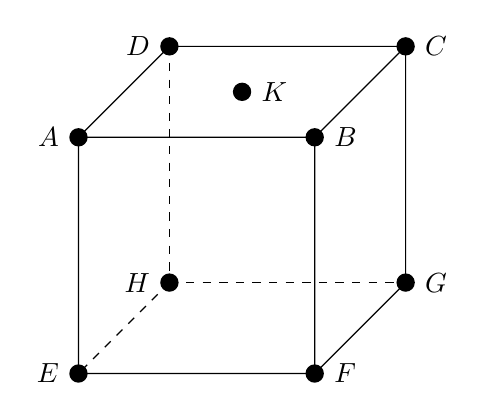
\begin{tikzpicture}[every edge quotes/.append style={auto, text=blue}]
    \pgfmathsetmacro{\cubex}{3}
    \pgfmathsetmacro{\cubey}{3}
    \pgfmathsetmacro{\cubez}{3}
    
    \pgfmathsetmacro{\cubeShiftX}{0} %做出平行六面體的傾斜感
    %%空間坐標中的CUBE 是以平面上的x軸 y軸再去擴充出深度z軸 z 往前為正,向後為負
    \coordinate (Eup1) at (0,0,0);
    \coordinate (Eup2) at (0,0,\cubez);
    \coordinate (Eup3) at (\cubex, 0, \cubez );
    \coordinate (Eup4) at (\cubex,0,0);
    \coordinate (Ecenter) at (0.5*\cubex , 0,0.5*\cubez);
    \coordinate (Edown1) at (\cubeShiftX+0, -\cubey, 0);
    \coordinate (Edown2) at (\cubeShiftX+0, -\cubey, \cubez);
    \coordinate (Edown3) at (\cubeShiftX+\cubex, -\cubey, \cubez);
    \coordinate (Edown4) at (\cubeShiftX+\cubex, -\cubey, 0); 
    \draw [draw=black, every edge/.append style={draw=black, dashed}]
    (Eup1) -- (Eup2) --(Eup3) --(Eup4) -- cycle
    (Eup3) -- (Edown3) -- (Edown4) -- (Eup4) --cycle
    (Eup2) -- (Edown2) -- (Edown3) -- (Eup3) --cycle 
    (Eup1) edge (Edown1) 
    (Edown1) edge (Edown4)
    (Edown1) edge (Edown2);
    
    \foreach \v/\u/\t in 
    {Eup1/180/$D$,
        Eup2/180/$A$,
        Eup3/0/$B$,
        Eup4/0/$C$,
        Edown1/180/$H$,
        Edown2/180/$E$,
        Edown3/0/$F$,
        Edown4/0/$G$,
        Ecenter/0/$K$
    }
    {
        \draw[ultra thick,fill] (\v) circle (2.5pt);
        \node[label=\u:\t] at (\v){};
    };     
    \end{tikzpicture}
    
    \begin{tikzpicture}[every edge quotes/.append style={auto, text=blue}]
    \pgfmathsetmacro{\cubex}{3}
    \pgfmathsetmacro{\cubey}{3}
    \pgfmathsetmacro{\cubez}{3}
    
    \pgfmathsetmacro{\cubeShiftX}{0} %做出平行六面體的傾斜感
    %%空間坐標中的CUBE 是以平面上的x軸 y軸再去擴充出深度z軸 z 往前為正,向後為負
    \coordinate (Eup1) at (0,0,0);
    \coordinate (Eup2) at (0,0,\cubez);
    \coordinate (Eup3) at (\cubex, 0, \cubez );
    \coordinate (Eup4) at (\cubex,0,0);
    
    \coordinate (Edown1) at (\cubeShiftX+0, -\cubey, 0);
    \coordinate (Edown2) at (\cubeShiftX+0, -\cubey, \cubez);
    \coordinate (Edown3) at (\cubeShiftX+\cubex, -\cubey, \cubez);
    \coordinate (Edown4) at (\cubeShiftX+\cubex, -\cubey, 0); 
    \coordinate (P) at ($(Eup2)!0.5!(Eup3)$);
    \coordinate (Q) at ($(Eup3)!0.5!(Eup4)$);
    
    \draw [draw=black, every edge/.append style={draw=black, dashed}]
    (Eup1) -- (Eup2) --(Eup3) --(Eup4) -- cycle
    (Eup3) -- (Edown3) -- (Edown4) -- (Eup4) --cycle
    (Eup2) -- (Edown2) -- (Edown3) -- (Eup3) --cycle 
    (Eup1) edge (Edown1) 
    (Edown1) edge (Edown4)
    (Edown1) edge (Edown2)
    (P) -- (Q) -- (Edown3) --cycle;
    
    
    \foreach \v/\u/\t in 
    {Eup1/180/$E$,
        Eup2/180/$F$,
        Eup3/225/$G$,
        Eup4/0/$H$,
        Edown1/180/$A$,
        Edown2/180/$B$,
        Edown3/0/$C$,
        Edown4/0/$D$,
        P/90/$P$,
        Q/0/$Q$
    }
    {
        \draw[ultra thick,fill] (\v) circle (2pt);
        \node[label=\u:\t] at (\v){};
    };     
    \end{tikzpicture}
    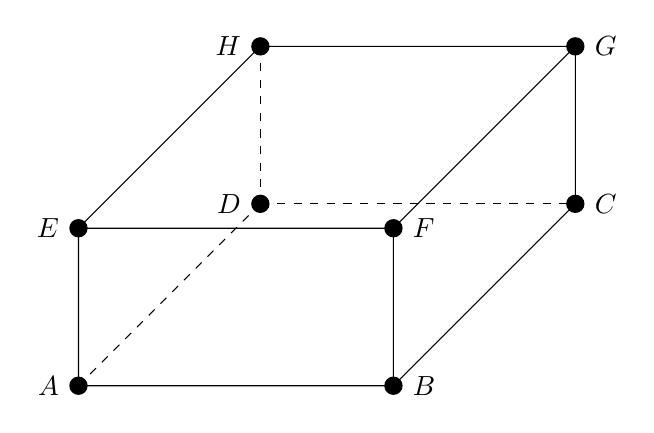
\begin{tikzpicture}[every edge quotes/.append style={auto, text=blue}]
    \pgfmathsetmacro{\cubex}{4}
    \pgfmathsetmacro{\cubey}{2}
    \pgfmathsetmacro{\cubez}{6}
    
    \pgfmathsetmacro{\cubeShiftX}{0} %做出平行六面體的傾斜感
    %%空間坐標中的CUBE 是以平面上的x軸 y軸再去擴充出深度z軸 z 往前為正,向後為負
    \coordinate (Eup1) at (0,0,0);
    \coordinate (Eup2) at (0,0,\cubez);
    \coordinate (Eup3) at (\cubex, 0, \cubez );
    \coordinate (Eup4) at (\cubex,0,0);
    \coordinate (Edown1) at (\cubeShiftX+0, -\cubey, 0);
    \coordinate (Edown2) at (\cubeShiftX+0, -\cubey, \cubez);
    \coordinate (Edown3) at (\cubeShiftX+\cubex, -\cubey, \cubez);
    \coordinate (Edown4) at (\cubeShiftX+\cubex, -\cubey, 0); 
    \draw [draw=black, every edge/.append style={draw=black, dashed}]
    (Eup1) -- (Eup2) --(Eup3) --(Eup4) -- cycle
    (Eup3) -- (Edown3) -- (Edown4) -- (Eup4) --cycle
    (Eup2) -- (Edown2) -- (Edown3) -- (Eup3) --cycle 
    (Eup1) edge (Edown1) 
    (Edown1) edge (Edown4)
    (Edown1) edge (Edown2);
    
    \foreach \v/\u/\t in 
    {Eup1/180/$H$,
        Eup2/180/$E$,
        Eup3/0/$F$,
        Eup4/0/$G$,
        Edown1/180/$D$,
        Edown2/180/$A$,
        Edown3/0/$B$,
        Edown4/0/$C$
    }
    {
        \draw[ultra thick,fill] (\v) circle (2.5pt);
        \node[label=\u:\t] at (\v){};
    };     
    \end{tikzpicture}
    
        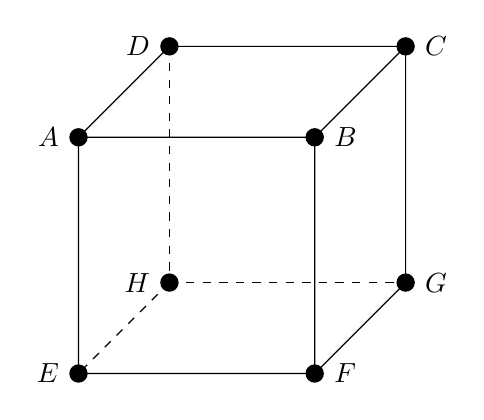
\begin{tikzpicture}[every edge quotes/.append style={auto, text=blue}]
        \pgfmathsetmacro{\cubex}{3}
        \pgfmathsetmacro{\cubey}{3}
        \pgfmathsetmacro{\cubez}{3}
        
        \pgfmathsetmacro{\cubeShiftX}{0} %做出平行六面體的傾斜感
        %%空間坐標中的CUBE 是以平面上的x軸 y軸再去擴充出深度z軸 z 往前為正,向後為負
        \coordinate (Eup1) at (0,0,0);
        \coordinate (Eup2) at (0,0,\cubez);
        \coordinate (Eup3) at (\cubex, 0, \cubez );
        \coordinate (Eup4) at (\cubex,0,0);
        \coordinate (Edown1) at (\cubeShiftX+0, -\cubey, 0);
        \coordinate (Edown2) at (\cubeShiftX+0, -\cubey, \cubez);
        \coordinate (Edown3) at (\cubeShiftX+\cubex, -\cubey, \cubez);
        \coordinate (Edown4) at (\cubeShiftX+\cubex, -\cubey, 0); 
        \draw [draw=black, every edge/.append style={draw=black, dashed}]
        (Eup1) -- (Eup2) --(Eup3) --(Eup4) -- cycle
        (Eup3) -- (Edown3) -- (Edown4) -- (Eup4) --cycle
        (Eup2) -- (Edown2) -- (Edown3) -- (Eup3) --cycle 
        (Eup1) edge (Edown1) 
        (Edown1) edge (Edown4)
        (Edown1) edge (Edown2);
        
        \foreach \v/\u/\t in 
        {Eup1/180/$D$,
            Eup2/180/$A$,
            Eup3/0/$B$,
            Eup4/0/$C$,
            Edown1/180/$H$,
            Edown2/180/$E$,
            Edown3/0/$F$,
            Edown4/0/$G$
        }
        {
            \draw[ultra thick,fill] (\v) circle (2.5pt);
            \node[label=\u:\t] at (\v){};
        };     
        \end{tikzpicture}
    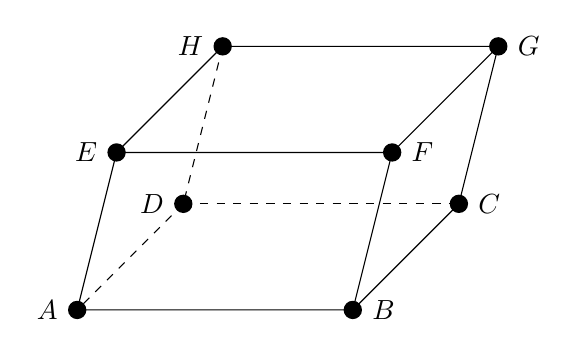
\begin{tikzpicture}[every edge quotes/.append style={auto, text=blue}]
    \pgfmathsetmacro{\cubex}{3.5}
    \pgfmathsetmacro{\cubey}{2}
    \pgfmathsetmacro{\cubez}{3.5}
    
    \pgfmathsetmacro{\cubeShiftX}{-0.5} %做出平行六面體的傾斜感
    %%空間坐標中的CUBE 是以平面上的x軸 y軸再去擴充出深度z軸 z 往前為正,向後為負
    \coordinate (Eup1) at (0,0,0);
    \coordinate (Eup2) at (0,0,\cubez);
    \coordinate (Eup3) at (\cubex, 0, \cubez );
    \coordinate (Eup4) at (\cubex,0,0);
    \coordinate (Edown1) at (\cubeShiftX+0, -\cubey, 0);
    \coordinate (Edown2) at (\cubeShiftX+0, -\cubey, \cubez);
    \coordinate (Edown3) at (\cubeShiftX+\cubex, -\cubey, \cubez);
    \coordinate (Edown4) at (\cubeShiftX+\cubex, -\cubey, 0); 
    \draw [draw=black, every edge/.append style={draw=black, dashed}]
    (Eup1) -- (Eup2) --(Eup3) --(Eup4) -- cycle
    (Eup3) -- (Edown3) -- (Edown4) -- (Eup4) --cycle
    (Eup2) -- (Edown2) -- (Edown3) -- (Eup3) --cycle 
    (Eup1) edge (Edown1) 
    (Edown1) edge (Edown4)
    (Edown1) edge (Edown2);
    
    \foreach \v/\u/\t in 
    {Eup1/180/$H$,
        Eup2/180/$E$,
        Eup3/0/$F$,
        Eup4/0/$G$,
        Edown1/180/$D$,
        Edown2/180/$A$,
        Edown3/0/$B$,
        Edown4/0/$C$
    }
    {
        \draw[ultra thick,fill] (\v) circle (2.5pt);
        \node[label=\u:\t] at (\v){};
    };     
    \end{tikzpicture}
    
    
    \begin{tikzpicture}[scale=0.6]
    \pgfmathsetmacro{\EAlphaVectorX}{8}
    \pgfmathsetmacro{\EAlphaVectorY}{0}
    \pgfmathsetmacro{\EBetaVectorX}{2}
    \pgfmathsetmacro{\EBetaVectorY}{3}
    \coordinate (cOPt) at (0,0);
    \coordinate (cPPt) at (3,1.5);
    \coordinate (cQPt) at (8,1.5);
    \coordinate (cVectorPP) at (0,3);
    \coordinate (cNVector) at (0,3); 
    \coordinate (cPPrimePt) at ($(cPPt)+(cVectorPP)$);
    \coordinate (cQPrimePt) at ($(cQPt)+(cVectorPP)$);
    \coordinate (cNVectorStartPt) at (1.5,1.5);
    \coordinate (cNVectorEndPt) at ($(cNVectorStartPt) + (cNVector)$);
    \coordinate (cLineStartPt) at (7,4);
    \coordinate (cLineVector) at (-2,-2.5);
    
    \coordinate (cAlphaPt) at  (\EAlphaVectorX, \EAlphaVectorY) ; 
    \coordinate (cLineEndPt) at ($(cLineStartPt) + 2*(cLineVector)$);
    \coordinate (cLineMidPt) at (intersection of cLineStartPt--cLineEndPt and cPPt--cQPt);
    \coordinate (cLineMidPt2) at (intersection of cLineStartPt--cLineEndPt and cOPt--cAlphaPt);
    
    
    \draw[ultra thick] (cPPt)--(cQPt);
    \draw (cPPrimePt)--(cQPrimePt);
    \draw[fill=lightgray] (cPPt)--(cQPt)--(cQPrimePt)--(cPPrimePt)--cycle;
    \draw (0,0) -- ++(\EAlphaVectorX, \EAlphaVectorY) -- ++(\EBetaVectorX, \EBetaVectorY) -- ++(-\EAlphaVectorX, -\EAlphaVectorY) -- ++(-\EBetaVectorX, -\EBetaVectorY) -- cycle;
    \draw (cPPt) -- ++(cVectorPP);
    \draw (cQPt) -- ++(cVectorPP) ;
    
    \draw[-{Stealth[scale=1.3,angle'=45]},semithick] (cNVectorStartPt) -- (cNVectorEndPt) ;
    
    \draw[ultra thick] (cLineStartPt)--(cLineMidPt);
    \draw[ultra thick,dashed] (cLineMidPt)--(cLineMidPt2);
    \draw[ultra thick] (cLineMidPt2)--(cLineEndPt);
    \foreach \v/\u/\t in 
    { cNVectorEndPt/90/$\lvec{n}$,
        cLineStartPt/180/$\Gamma$,
        cQPrimePt/0/$E_2$
    }
    {
        %\draw[ultra thick,fill] (\v) circle (2.5pt);
        \node[label=\u:\t] at (\v){};
    };
    \draw[ultra thick,fill] (cLineMidPt) circle (2.5pt);
    \node[below] at (8,0){$E_{xy}$};
    %       
    \end{tikzpicture}